\section{Reflection High-Energy Electron Diffraction}
After a thin film has been deposited, it is crucial to examine its crystal structure. 
To get information regarding the surface crystal quality, a \ac{rheed} experiment 
can be performed. 
Grazing incidence electrons are focused onto the sample's surface, where they undergo 
diffraction and are subsequently captured by a detector.
In the following sections, the design of a \ac{rheed} chamber as well as
its basic working principles shall be explained.
This chaption is based on the work of \cite{rheed}.

\subsection{Design of a \ac{rheed} System}

\begin{figure}
    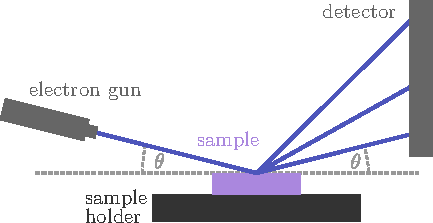
\includegraphics{../assets/rheed.pdf}
    \caption{Schematic setup of the main \ac{rheed} components. \imcitetwo{wikimedia}}
	\label{fig:rheed_1}
\end{figure}

A schematic setup of a \ac{rheed} system is depicted in \cref{fig:rheed_1}.
The main components are an electron gun and a photoluminescence detector. 
The electron gun generates an electron beam that strikes the sample at a very small 
angle, typically between \qtyrange{0.5}{2.5}{\degree} relative to the sample's surface. 
The incident electrons diffract on the surface and are caught on a photoluminescence 
screen. 
The resulting diffraction pattern provides conclusions about the surface crystal 
structure. 
To get accurate results, a clean surface is necessary.

The most important device of the \ac{rheed} setup is the electron gun.
A thermionic cathode, typically made of tungsten, is negatively biased and emits 
electrons.
Those electrons are accelerating through a positively biased anode, whereby the anode
bias determines the electron energy that is typically between 
$\qty{10}{\kilo\electronvolt}$ and $\qty{30}{\kilo \electronvolt}$.
The optimal anode bias depends on the desired information.
On the one hand, high-energetic electrons penetrate the surface of the sample deeper, 
resulting in a degradation of the surface sensitivity.
On the other hand, more information is recorded for high energies, as the Laue
zones are proportional to the inverse square of the electron energy. 
This leads to a decrease of stray field influence as well. 
To avoid unwanted scattering of the electrons with gas molecules, the \ac{rheed} system 
is operated under high-vacuum conditions.

The electron beam is focused by a magnetic and an electric lens system, such that
the focal point is located on the detector.
Photoluminescence screens that emit green light when 
electrons hit their surface, are widely used as detectors.
To capture the diffraction pattern for digital analysis, a CCD camera is used. 
Single channel detectors are also applicable to obtain high-sensitive intensity data.

\subsection{Working Principles}
The surface atoms of the sample diffract the incident electron beam.
A diffraction pattern (points on photoluminescence screen) 
is generated as a function of the crystal structure.
A suitable approach to model this system is the kinematic scattering theory, 
that will be elaborated in the next chapter. 

\subsubsection{Kinematic Scattering Theory}
The incident electron beam can be characterized using the wavevector $\mathbf{k}_{0}$,
the diffracted beam with $\mathbf{k}'$.
In kinematic scattering theory, only one elastic scattering event per particle is 
assumed. 
The term 'elastic' states that the energy $E$ and thus the magnitude of the wavevector
of the incident and diffracted beam is equal.
This can be expressed analytically with:
\begin{equation}
	\lvert \mathbf{k}' \rvert=\lvert \mathbf{k}_{0} \rvert
\end{equation}
Every crystal lattice can be described by a set of reciprocal lattice vectors
$\mathbf{G}$. 
A crystal lattice diffraction is only possible, if it obeys the Laue condition:
\begin{equation}
\mathbf{k}'-\mathbf{k}_{0}=\mathbf{G}
\end{equation}
In a \ac{rheed} experiment, the incident beam angle can be obtained using the 
geometry of the setup.
The diffracted beam angle corresponds to the angle between the sample's surface  and the 
vector pointing to a diffraction spot on the detector. 
Incident and diffracted beam energies are equal and specified by the electron gun.
Therefore, the reciprocal lattice vectors can be reconstructed using a \ac{rheed} 
pattern. 

\ac{rheed} is a very surface-sensitive technique, as it only samples a few atomic layers 
beneath the surface.
The surface-normal component $k_{0z}$ can be varied by changing the incidence angle 
$\theta$ and is usually low, typically around \qty{1}{\kilo \electronvolt}.
The crystal structure can thus be approximated by a two-dimensional surface lattice.
This differs from the reciprocal lattice of a three-dimensional bulk crystal.
Instead of well-defines reciprocal lattice points, the reciprocal lattice degenerates 
into one-dimensional rods extending perpendicular to the sample's surface, as depicted 
in \cref{fig:rheed_2}.
Each rod can be characterized by two indices $h$ and $l$, in contrast to the three 
indices $h$, $k$ and $l$ of a bulk crystal.

To account for the degeneracy, the reciprocal space vectors $\mathbf{G}_{hl}$ are only 
defined inside the surface plane and originate from the two-dimensional direct lattice
of the surface. 
If $\hat{P}$ is the projection operator onto the surface plane, the Laue condition can 
be rewritten as:
\begin{equation}
	\mathbf{G}_{hl}=P(\mathbf{k}_{hl}-\mathbf{k}_{i})
\end{equation}

To find reciprocal lattice parameters, it is useful to construct the Ewald sphere.
The Ewald sphere is centered on the sample surface and has a radius 
$\lvert \mathbf{k}_0 \rvert$.
It shows allowed diffraction conditions for kinematically scattered electrons.
Diffraction occurs for all $\mathbf{k}'$ if:
\begin{itemize}
	\item $\mathbf{k}'$ is on the Ewald sphere
	\item $\mathbf{k}'$ intersects with translated reciprocal space rods that extending
		perpendicular to the sample surface at $\mathbf{G}_{hl}+\mathbf{k}_{0}$
\end{itemize}

Due to the high energy electrons, the Ewald sphere is large.
For a typical energy of \qty{20}{\kilo \electronvolt}, the radius is
approximately \num{70} times larger than the reciprocal lattice unit of \ce{GaAs}.
As a result, it intersects with multiple reciprocal lattice rods. 
These rods can be organized into Laue planes.
The intersection of the Ewald sphere with a Laue plane is called a Laue circle.
Of particular interest are Laue planes, that are parallel to the detector surface.
The resulting Laue circles are projected as concentric circles on the detector
and can be labeled beginning from the center outwards with $n=0,1,2,\ldots$.
The \ac{rheed} pattern can therefore be interpreted as a collection of Laue circle 
points that are projected onto the detector.
All circles are centered around the specular point, which is the projection of the 
intersection of the Ewald sphere with the $(00)$ rod.
The specular spot has the greatest intensity of the \ac{rheed} pattern and its angle
with the substrates surface is equal to the incident electron beam angle.
For each circle, the corresponding radius $L_{n}$ can be measured as 
well as the horizontal distance $l$ between two adjacent points on the same circle.
With some trigonometric consideration and the quantities depicted in \cref{fig:rheed_2},
the lattice parameters can be calculated as follows:

\begin{align}
n g_{\perp} &=\frac{k_{0}}{\sqrt{ (L/nl)^{2}+1 }} \\
ng_{\parallel} &= k_{0} \left[ \cos\theta-\frac{1}{\sqrt{ (L_{n} / L)^{2}+1 }} \right]
\end{align}

The sample can be rotated around the surface normal to obtain different
\ac{rheed} patterns.
If the direct lattice is rotated, the reciprocal lattice is rotated as well.
Every rotation symmetry of the direct lattice is a symmetry of the reciprocal 
lattice.
\ac{rheed} scans for different azimuth angles can therefore be used to determine 
surface lattice rotational symmetries.   
Sample rotation is also useful to optimize the intensity of the \ac{rheed} pattern.

\subsubsection{Dynamic and Inelastic Scattering Influence}
Kinematic scattering theory is a good approximation for \ac{rheed}, 
because the majority of the electrons are elastically scattered.
However, multiple elastic collisions per particle (dynamic scattering) are possible and
therefore complicate the analysis. 

Inelastic scattering events occur as well, where the energy of the incident electrons 
is not conserved during the scattering process.
This is primarily caused by plasmon excitations, which are collective oscillations of
charge density waves inside the sample.
The electrons lose energy and change their direction.
As a result, the reflection profiles are broadened. 

Other inelastic scattering events include, but are not limited to: band-to-band 
transitions, atomic core-shell excitations and phonon scattering.

\subsection{Comparison to XRD}
\ac{rheed} and \ac{xrd} are two distinct measurement techniques that originate from
the same physical principles. 
Both techniques utilize the Laue diffraction condition that provides insight into 
the reciprocal lattice crystal structure. 
With that, it is possible to determine the lattice parameters and the crystal symmetry,
usually of thin films.
However, the two techniques differ in their underlying physics as well as their primary 
purposes of use.

The main difference between \ac{rheed} and \ac{xrd} is the utilized type of radiation.
\ac{rheed} uses high-energy electrons, while \ac{xrd} uses X-rays.
A \ac{rheed} experiment has to be performed under high-vacuum conditions, as the 
electrons would be scattered by gas molecules.
\ac{xrd} experiments can be performed in air, as the X-rays are not significantly
scattered by air molecules.

In \ac{rheed}, the electron beam is focused on the sample surface at a very small angle,
such that only a few atomic layers are probed.
In contrast, \ac{xrd} is not restricted to a small incidence angle and can be used to
analyze bulk crystal structures as well.

Due to the different sample depths, the diffraction pattern as well as the reciprocal
lattice structure differ.
The reciprocal space obtained by \ac{rheed} is a two-dimensional surface lattice, that
degenerates into one-dimensional rods along the surface normal.
In \ac{xrd}, the reciprocal space is the ordinary three-dimensional point lattice.

Usually a photoluminescence screen is used as a detector in \ac{rheed} systems that 
enables only a quantitative analysis of the diffraction pattern position.
Semiconductor detectors are used in \ac{xrd} systems, which allow for a quantitative
analysis of the intensity of the diffraction pattern. 

In a \ac{rheed} experiment, the sample can be rotated only around the surface normal.
In contrast, \ac{xrd} experiments allow for consecutive sample rotations around multiple
axes as well as translations, due to a goniometer setup. 

\subsection{In Situ RHEED} \label{sec:in_situ_rheed}
A popular application of \ac{rheed} is in situ monitoring of thin film growth, 
especially in \ac{mbe} systems.
In this setup, the \ac{rheed} system is integrated into the \ac{mbe} chamber, 
and the \ac{rheed} pattern is recorded during the growth process.
The intensity of individual spots is monitored and fluctuates 
in a periodic manner.
These fluctuations are called \ac{rheed} oscillations and can be used to determine the
flux of the target species in \ac{mbe} systems.
Each maximum of the \ac{rheed} oscillation corresponds to the growth of 
a complete monolayer.

\begin{figure}
    \centering
    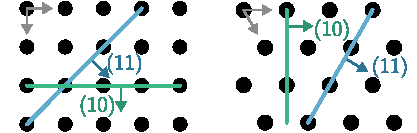
\includegraphics{../assets/planes.pdf}
	\caption{Observed Laue planes}
	\label{fig:planes}
\end{figure}

\begin{figure*}
	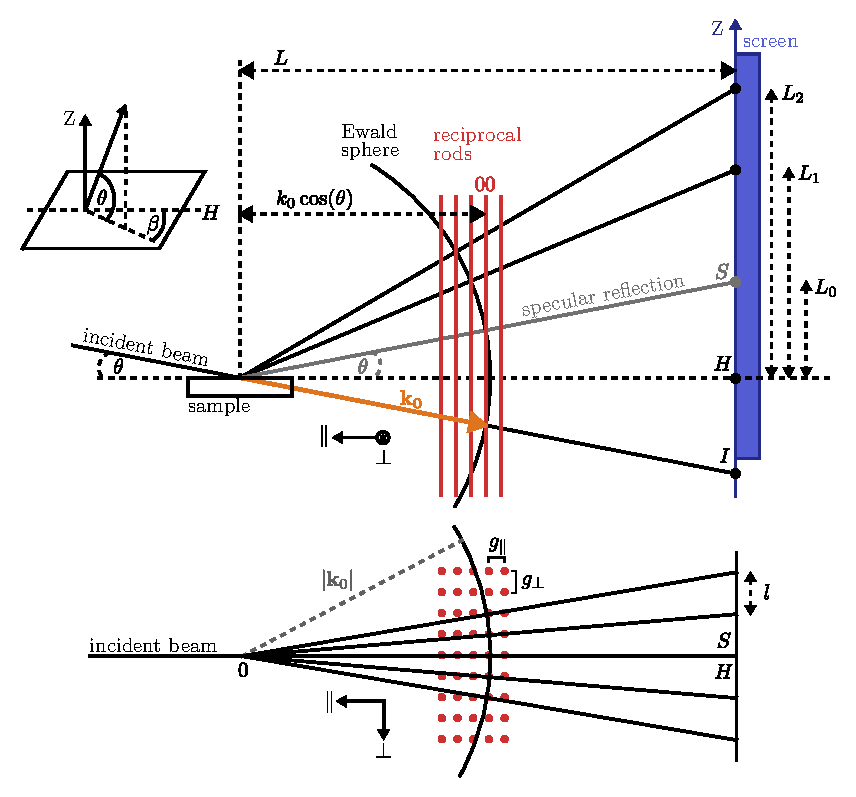
\includegraphics{../assets/rheed_2.pdf}
	\caption{Schematic representation of the Ewald sphere and the reciprocal lattice
	in \ac{rheed} experiments. }
	\label{fig:rheed_2}
\end{figure*}

